\chapter{{Wprowadzenie do technik ekstracji częstotliwości podstawowej}}
\label{chapter:przeglad}
\thispagestyle{empty}

W tym rozdziale zostaną przedstawione istniejące rozwiązania służące do wykrywania wysokości dźwięku oraz aplikacje dające możliwość sterowania kontrolerami MIDI za pomocą wysokości dźwięku. W zestawieniu znajdą się wybrane aplikacje komercyjne, które cieszą się największą popularnością. Przeanalizowane zostaną również istniejące środowiska programistyczne.

\section{{Mechanizmy identyfikacji wysokości dźwięku}}
 W pierwszej części aplikacji podany na wejściu dźwięk zostanie poddanie analizie za pomocą wybranego algorytmu do estymacji tonu prostego. Następnie uzyskany rezultat zostanie użyty do wygenerowania dźwięku w formacie MIDI. Poniżej został przedstawiony prosty schemat obrazujący przebieg działania aplikacji.
 
 
 \begin{figure}[h!]
  \centering
  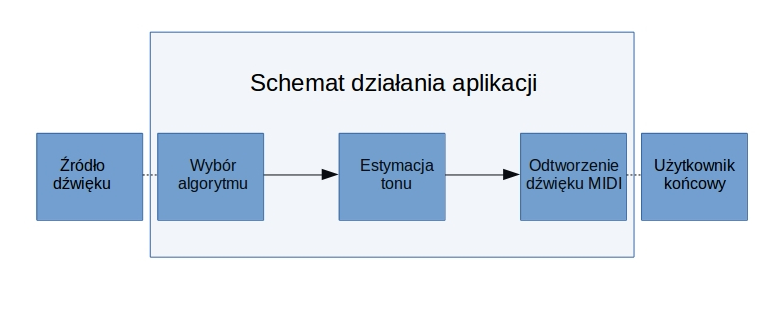
\includegraphics[width=0.5\linewidth]{rys/schematAplikacji}
  \caption{Schemat działania aplikacji.}
  \label{fig:schemat}
\end{figure}


W jednym z pierwszych etapów przedstawionym na schemacie jest wybór odpowiedniego algorytmu. Algorytmy do wykrywania tonu prostego już istnieją i do realizacji tej pracy inżynierskiej nie ma potrzeby tworzenia nowych. Z istniejących rozwiązań do realizacji zadania zostały wykorzystane algorytmy:

\begin{itemize}
\item[•]{\cite{YIN}YIN jest algorytmem zawierającym kilka pożądanych cech, które zdecydowały o jego użyciu w aplikacji. W głównej mierze bazuje na metodzie autokorelacji z niewielkimi modyfikacjami pozwalającymi uniknąć błędów. Nie ma górnego ograniczenia częstotliwośći, przez co jest odpowiedni dla wysokich dźwięków oraz muzyki. Jego realizacja jest stosunkowo prosta i wystarczająco wydajna przy niewielkim opóźnieniu}

\item[•]{\cite{harvey}MPM (ang. McLeod Pitch Method) jest algorytmem również bazujący na metodzie autokorelacji. Może działać w czasie rzeczywistym ze standardowym próbkowaniem 44.1 kHz. Działa bez zastosowania filtra dolnoprzepustowego i może pracować z dźwiękiem o wysokiej harmonicznej jak np. dźwięk generowany przez skrzypce. Rejestrowane zmiany przez ten algorytm mają niezawodną dokładność 1 centa. MPM działa również dobrze bez przetwarzania końcowego poprawy wysokości dźwięku, co jest powszechnie stosowane w przypadku innych algorytmów.}

\item[•]{\cite{harvey}Dynamic Wavelat jest to algorytm, który do wyznaczania wysokości tonu używa tz. falki. Wykorzystuje on STFT (ang. Short-time Fourier transform) oraz okna o stałeś liczbie oscylacji. Długość okna określa się jako stałą liczbę okresów w tej częstotliwości.}

\item[•]{\cite{AMDF} AMDF (ang. Average  Magnitude Difference Function) używa metody, która jest odmianą autokorelacji. Algorytm, zamiast korelować dane wejściowe przy różnych opóźnieniach (gdzie multiplikacje i podsumowania są tworzone dla każdej wartości) tworzy sygnał różnicowy pomiędzy dźwiękiem opóźnionym a oryginalnym i dla każdej wartości opóźnienia przyjmowana jest wartość bezwzględna.}

\end{itemize}
 


Metoda autokorelacji wykorzystana w algorytmach YIN oraz MPM można obliczyć ze wzoru:
\begin{equation}
\label{equation:2}
   Rxx(n) = \sum_{m=0}^{M-1}{x(m)x(m+n)}
\end{equation}
Gdzie $Rxx$ jest dyskretną autokorelacją o opóźnieniu $l$, a $x(m)$ jest sygnałem dyskretnym.

Do wyznaczenia częstotliwości możemy również wykorzystać DFT(ang. Discrete Fourier Transform), która możena obliczyć ze wzoru:
\begin{equation}
\label{equation:3}
   Rxx(n) = \sum_{n=0}^{N-1}*{x(n)}*e^{-{j2 \pi nk}/{N }},  n \in{\mathbb{Z}}
\end{equation}
Gdzie $j$ to jednostka urojona,$k$ to numer harmonicznej, $n$ to numer próbki sygnału,$N$ to liczba próbek.



 Dla algorytmu Dynamic Wavelat należy użyć metody CWT(ang. Continuous Wavelet Transform) danej wzorem:
\begin{equation}
\label{equation:1}
    c(a, b) = \int f(t) \Psi (at + b)dt
\end{equation}
Gdzie wartość  $c(a, b)$ jest współczynnikiem CWT  obliczonym poprzez splatanie sygnału $f(t)$ z falką, $\Psi$, skala $a$ o przesunięciu $b$ w czasie.
CWT często odnosi się do wektora wszystkich współczynników dla danej skali.
Podczas przetwarzania dużych sygnałów lub wielowymiarowych sygnałów, nadmiarowe dane sprawiają, że proces nie będzie możliwy do obliczenia. Wprowadzona została również Szybka transformacja falkowa (FWT)(ang. Fast Wavelet Transformation). FWT eliminuje problem nadmiarowości dięki wykorzystaniu ortogonalności. Para funkcji jest ortogonalna, jeżeli ich wewnętrzny produkt wynosi zero. Oznacza to, że każda informacja zakodowana przez pierwszą falkę nie jest zakodowana przez drugą i odwrotnie. Zatem nie traci  się czasu na obliczanie nadmiarowych danych.


\section{{Przegląd istniejących aplikacji}}
Pierwszym z najbardziej popularnych programów nawiązujących do tematyki pracy jest program o nazwie „Jam Origin”. 


\begin{figure}[h!]
  \centering
  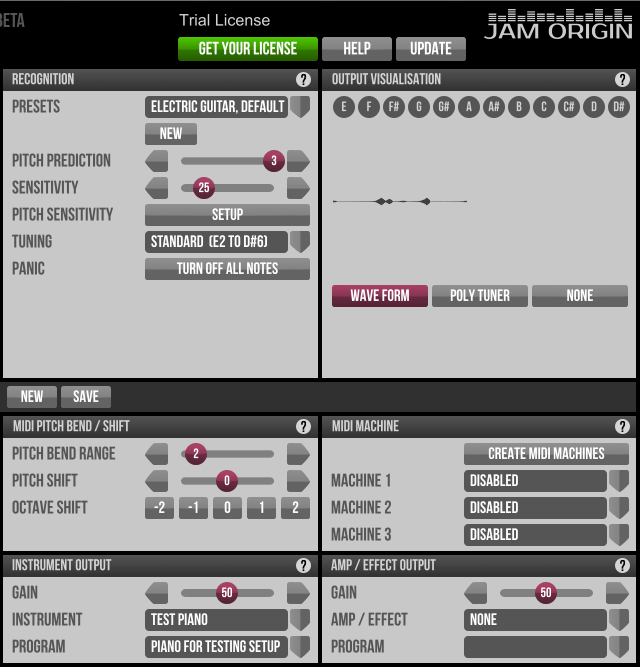
\includegraphics[width=0.5\linewidth]{rys/jamOrigin1}
  \caption{Zrzut ekranu z aplikacji Jam Origin.}
  \label{fig:schemat}
\end{figure}


Głównymi zaletami aplikacji są rozbudowane funkcje konfiguracji, jako że budowa instrumentów znacząco różni się ze względu na podział np.: smyczkowe, dęte. W większości przypadków można skonfigurować aplikacje pod daną kategorię, poczynając od instrumentów wydobywających pojedynczy dźwięk, aż po instrumenty wytwarzające kilka dźwięków jednocześnie. Najbardziej trafnym przykładem odnoszącym się do instrumentów wytwarzających kilka dźwięków jest gitara elektryczna. Aplikacja „Jam Origin” pozwala na jawne rozdzielenie kilku zagranych dźwięków lub wybieranie trybu mapowania tylko pojedynczego dźwięku. Ma to szczególne znaczenie przy dokładności i wierności odtwarzania wysokości tonów. Program ma też takie funkcje jak czułość przechwytywania dźwięku, co powoduje rzadsze pojawianie się błędów i daje możliwość dopasowania aktualnego poziomu wzmocnienia na wejściu do czułości przechwytywania.


Kolejnym wartym uwagi programem, zaliczającym się do aplikacji konwertującej dźwięk na  MIDI  jest „ Migic”. Zasada działania aplikacji jest podobna do poprzedniego przykładu, lecz główną różnicą pomiędzy tymi programami jest zbiór funkcji udostępniony użytkownikowi. Mianowicie „Migic” posiada wszystkie funkcje poprzednika oraz dodatkowo udostępnia pokaźną liczbę informacji.

\begin{figure}[h!]
  \centering
  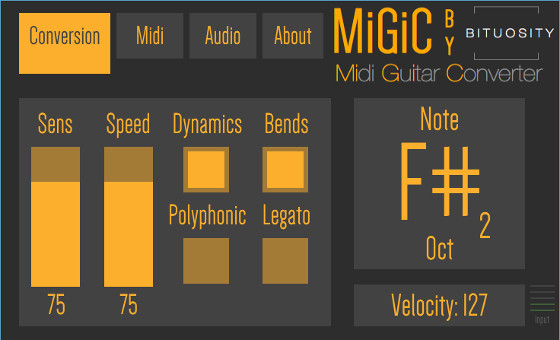
\includegraphics[width=0.5\linewidth]{rys/MIGIC1}
  \caption{Zrzut ekranu z aplikacji MiGiC.}
  \label{fig:schemat}
\end{figure}

Do najważniejszych z nich zaliczą się: informacja o opóźnieniu pomiędzy zagranym dźwiękiem, a jego odpowiednikiem w interfajsie MIDI.
Również przydatną informacją jest wyświetlanie tonacji aktualnie granych dźwięków w formie graficznej. Ponadto program udostępnia różnego rodzaju efekty takie jak, pogłosy, echo, zmianę tonacji dźwięku w czasie rzeczywistym.
Przedstawione programy są jednymi z najbardziej popularnych programów komputerowych nawiązujących tematyką do tej pracy. Istotnym faktem jest to, iż na rynku istnieje jeszcze kilka rozwiązań konwersji dźwięku na MIDI. Jednakże są to rozwiązania rozbieżne z tematem pracy, ponieważ są w dużej mierze realizowane na poziomie sprzętowym z dedykowanymi programami na systemy wbudowane.


\section{{Standard MIDI}}

\cite{MIDI} Standard MIDI jest to format u standaryzowany w 1983 roku. Format plików nie zawierają bezpośrednio zapisu dźwięku. Zawierają szereg informacji, za pomocą których możemy uzyskać dźwięk na urządzeniu obsługującym ten format. Odgrywane sekwencje w postaci programowej można przyrównać do zapisu nutowego lub do pozytywek na taśmy perforowane. W formie sekwencji zapisywane są polecenia note on oraz note off. Każdemu z tych poleceń przypisane są informacje w postaci atrybutów tj.

\begin{itemize}
\item[•]{key velocity zawiera informacje o sile nacisku na konkretny klawisz syntezatora,}
\item[•]{wysokość tonu,}
\item[•]{modulacja dźwięku,}
\item[•]{clock jest to informacja na temat synchronizacji czasowej pomiędzy poszczególnymi dźwiękami,}
\end{itemize}

Za pomocą tych informacji urządzenie jest w stanie odtworzyć sekwencje poleceń.  MIDI jest dość starym standardem, jednak jego specyfikacja nie uległa zmianie, przez co zachowuje pełną kompatybilność ze wszystkimi urządzeniami obsługującymi ten standard. Aktualnie standard MIDI jest wykorzystywany do sterowania różnego rodzaju syntezatorami i samplerami, w tym także wirtualnymi. W przypadku tej pracy inżynierskiej wykorzystywany będzie syntezator wirtualny. 


Istotną kwestią w pracy z  MIDI jest opóźnienie. Występuje ono w komunikacji pomiędzy sekwencerem MIDI, czyli w tym wypadku pierwszej części aplikacji, która odpowiedzialna jest znalezienie wysokości tonu i przesłanie go komunikatem MIDI, a urządzeniem odbiorczym, w tym przypadku druga część aplikacji odpowiadająca za odtwarzanie dźwięku. Na opóźnienie składa się również czas, jaki potrzebny jest na przetworzenie komunikatu w urządzeniu odbiorczym.


W standardzie MIDI występują kanały. Każdy kanał może zawierać inną treść podczas transmisji. Przykładowo na każdym kanale można przesyłać różne identyfikatory instrumentów oraz odpowiednie dla nich sekwencje pojedynczych nut lub ich zbiorów. Ważną rzeczą w tym założeniu jest fakt, iż tak naprawdę na stacji odbiorczej do każdego kanału dopasowuje się konkretny instrument. Odtworzony dźwięk będzie oczywiście brzmiał inaczej jeżeli np. na kanale zawierającym partię perkusyjne ustawiony zostanie np. fortepian. Podczas komunikacji pomiędzy różnymi urządzeniami należy zatem za każdym razem sprawdzić, czy ustawienia kanałów są zgodne z pierwowzorem. Problemy te związane były między innymi z różnicami wynikającymi z brakiem współpracy producentów. Jest to problematyczne jednak aktualnie w większości przypadków urządzenia  oraz programy wykorzystujące MIDI używają standardu General MIDI.


Standard ten został wprowadzony w 1991 roku. Jego założenia miały na celu usystematyzowanie dostępnych instrumentów, ponieważ kontrolowanie ustawień konkretnych instrumentów na danych kanałach zdecydowanie zaburzało łatwość komunikacji. Został wprowadzony bank 128 brzmień. General MIDI obligował producentów i twórców oprogramowania do zachowania kompatybilności dźwięku instrumentów czy efektów. Dla przykładu na pierwszych sześciu pozycjach znajdują się wariacje dźwięku pianina, następnie organ, gitar oraz instrumentów basowych. Oprócz u standaryzowania instrumentów zostały także postawione wytyczne co do wysokości tonów dla instrumentów perkusyjnych. Obsługa zwiększonej liczby instrumentów nadal pozostaje kompatybilna ze standardem zapisu SMF.


SMF (ang. Standard MIDI Files) - Standard jednolitego zapisu informacji dla sekwencerów. Pomimo iż każda firma do swojego sprzętu oraz aplikacji bazujących na MIDI, używa swojego specjalistycznego sposobu zapisu danych, większość urządzeń oraz aplikacji obsługuje standard SMF. Sytuacja ma się inaczej w przypadku dodatkowych informacji dostępnych tylko i wyłącznie dla konkretnych modeli urządzeń lub serii produktów, w skład którego również wchodzi oprogramowanie. Informacje te zostają utracone. Nie wpływa to na odtwarzany dźwięk na urządzeniu końcowym.
Zostały utworzone trzy wersje formatu SMF, oznaczone kolejno 0, 1, 2 . W chwili pisania pracy standard jest nadal w użytku i służy do wymiany informacji pomiędzy urządzeniami i  aplikacjami obsługującymi format MIDI. W użytku pozostaje wersja 0 oraz 2. Głównymi różnicami pomiędzy tymi dwoma wydaniami standardu SMF jest sposób zapisu. Dla formatu oznaczonego numerem 0 zapis odbywa się na jednej ścieżce. Jest to dopuszczalny sposób ze względu na to, iż każde zdarzenie MIDI ma w sobie zawartą informację o numerze kanału. Po załadowaniu pliku zapisanego w formacie SMF w wersji 0, urządzenie odbiorcze może bez problemu rozdzielić pojedynczą ścieżkę na wiele ścieżek. Jest to pewna niedogodność, która nie występuje w przypadku wersji 1. W tym wariancie plik zawiera informacje MIDI w formacie wielościeżkowym. Zaletą tego jest niewątpliwie to, że załadowany plik jest bezpośrednio gotowy do użycia lub edycji.


Przykładowa wizualizacja zapisu formatu MIDI w programie FL Studio.

\begin{figure}[h!]
  \centering
  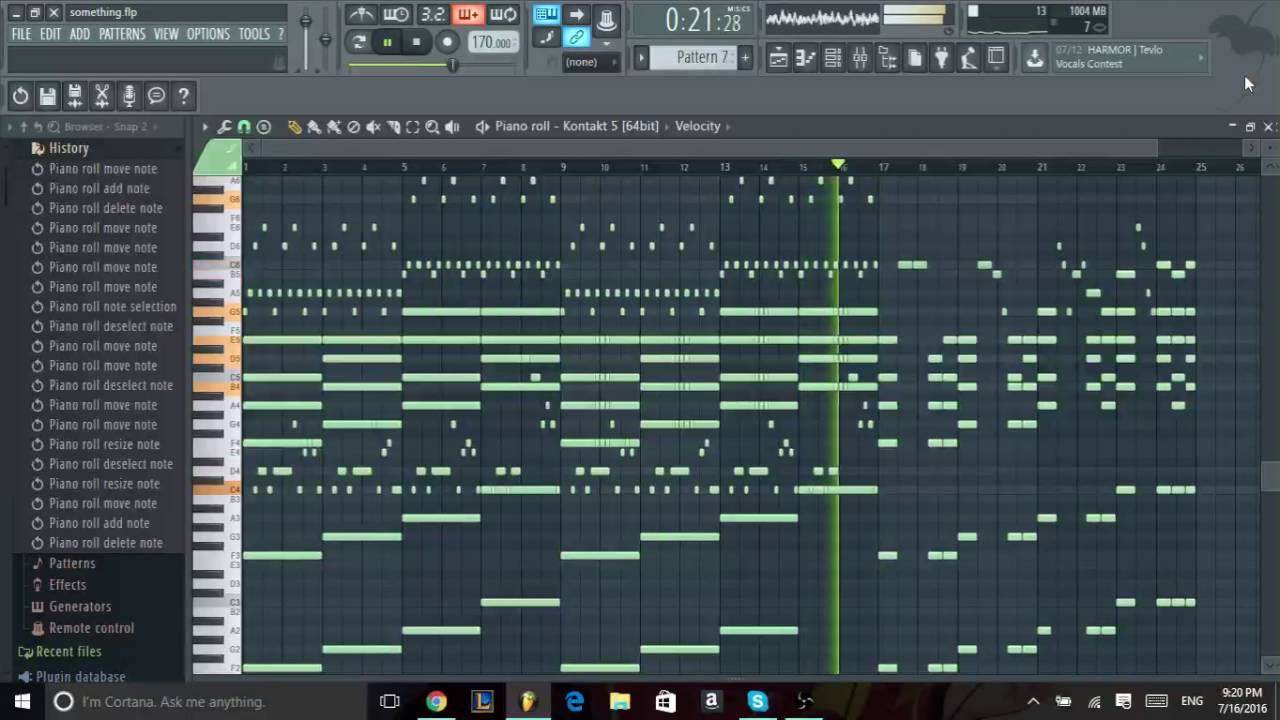
\includegraphics[width=0.5\linewidth]{rys/fl1}
  \caption{Zrzut ekranu z aplikacji FL Studio.}
  \label{fig:schemat}
\end{figure}


Synchronizacja MIDI jest potrzebna, aby przeprowadzić poprawną komunikację pomiędzy urządzeniami obsługującymi interfejs MIDI. Jest to jeden z fundamentalnych aspektów współpracy urządzeń oraz aplikacji. Jednym ze sposobów synchronizacji jest MIDI Sync (MIDI Clock). W tym rodzaju synchronizacji brane są pod uwagę następujące komunikaty:


\begin{itemize}
\item[•]{"Start", komunikat ten zawiera informacje do urządzenia odbiorczego o rozpoczęciu odtwarzania.}
\item[•]{"Stop", komunikat ten zawiera informacje do urządzenia odbiorczego o zatrzymaniu odtwarzania.}
\item[•]{"Continue", komunikat ten zawiera informacje do urządzenia odbiorczego o odtwarzania od wskazanego miejsca.}
\item[•]{"Song Position Pointer", jest to komunikat nakazujący urządzeniu podrzędnemu zmianę w odtwarzaniu do określonego miejsca w utworze.}
\end{itemize}

Opis procesu synchronizacji wygląda następująco. Urządzenie wysyłające przekazuje informacje do urządzenia odbiorczego, w której zawarty jest komunikat zegarowy pracujący z częstotliwością 24 impulsy na ćwierć nutę. Oczywiście wynika z tego faktu zależności całego procesu od nadanego w utworze tempa. W przypadku gdy główny sekwencer zmieni tempo, zaczyna wysyłać większą liczbę impulsów na sekundę. Powoduje to zmianę tempa w urządzeniu odbiorczym.


Istnieje także inna metoda synchronizacji (ang. MIDI Time Code). Swoje główne zastosowanie znalazła dla obsługi przypadków, w których występuje potrzeba synchronizacji dźwięku oraz obrazu.  W tym typie synchronizacji należy odnieść się do czasu rzeczywistego wyrażonego w jednostkach: godzinach, minutach, sekundach. Jest to typ synchronizacji SMPTE, który nagrywany jest na osobnych ścieżkach rejestratora. Wykorzystuje generator kodu czasowego. Dzięki zastosowaniu oznaczeń czasowych, urządzenie odbiorcze jest w stanie zsynchronizować się w każdym momencie trwania utworu. Aby w moc wykorzystać oznaczenia czasowe, należy wyposażyć urządzenia w konwertery (sprzętowe lub programowe), które potrafią przetwarzać kod SMPTE na MIDI Time Code (MTC). Jest to kod spełniający funkcję analogiczną do powyższego, z tą różnicą, że nie pracuje w oparciu o sygnał audio. Kod MTC wykorzystuje specjalne komunikaty MIDI. Urządzenie odbiorcze po otrzymaniu komunikatu na, którym swoją pracę opiera MTC, ma za zadanie zamiana tych informacji na takty, bity oraz impulsy zegara są adekwatne do odpowiadających im jednostek czasu rzeczywistego. Powyższe rozwiązania nie są jednak na tyle dokładne, aby były wykorzystywane osobno do profesjonalnych zastosowań. Do takich zastosowań wykorzystywany jest Word Clock. Jest to sygnał zegarowy, który jest w pełni kompatybilny z pojedynczym impulsem próbkującym. 



\section{{Środowiska programistyczne}}

Aktualnie istnieje wiele rozbudowanych zintegrowanych środowisk programistycznych. Jednakże dla każdego istnieje uzasadnione przeznaczenie.

\begin{itemize}
\item[•]{Xcode,}
\item[•]{Eclipse,}
\item[•]{Netbeans.}
\end{itemize}


\cite{Xcode} jest zintegrowanym środowiskiem programistycznym stworzonym przez firmę Apple Inc. Wykorzystywana jest do tworzenia oprogramowania różnego rodzaju na systemy operacyjne OS X. Posiada rozbudowane funkcje: edycji plików, nawigacji po projekcie oraz  debugowania wszystkich typów projektów programistycznych OS X, włączając w to aplikacje, narzędzia, schematy, biblioteki, pakiety pluginowe, rozszerzenia jądra i sterowniki urządzeń. Xcode współpracuje także z systemem kontroli wersji Git poprzez zintegrowane funkcjonalności i specjalne przeznaczone do tego interfejsy dostępne dla programisty. Wszystkie potrzebne komendy zostały opatrzone w przyjazny dla użytkownika interfejs graficzny, co znacznie upraszcza zarządzanie projektem.


\cite{netbeans}Kolejne IDE, które cieszy się dużą popularnością to NetBeans. Jest to środowisko udostępnione bezpłatnie na większość dostępnych systemów operacyjnych. Środowisko to posiada szereg zalet i można uznać je za jedno z najlepszych środowisk programistycznych. Jest oficjalnym środowiskiem programistycznym dla Javy w wersji 8. NetBeans jako darmowe IDE jest przygotowane w kilku wersjach, przeznaczonych do różnych języków programowania. Edytor wspiera wiele składni języków takich jak:  Java, C/C++, XML, HTML, PHP, GROOVY, Javadoc i JavaScript. Edytor tego środowiska jest bardzo elastyczny i pozwala na rozszerzenie wsparcia dla większej liczby języków. Posiada również mechanizm uzupełniania składni oraz całych konstrukcji takich jak: wyrażenie warunkowe, pętle, instrukcje warunkowe. W przypadku pracy z dużym projektem  twórcy IDE udostępnili efektywne i proste w obsłudze narzędzia do zarządzania.


\cite{eclipse}Wybrane środowisko do tworzenia aplikacji to Eclipse. Jest to platforma programistyczna istniejąca od 2004 r. oparta na języku Java. Głównym powodem wyboru tego IDE, jest prostota użytkowania. Kolejnym argumentem, który przemawia za wyborem tego środowiska jest między innymi fakt, iż jest to najbardziej rozbudowane środowisko. Przygotowany jest do pracy z kilkoma językami programowania w zależności od wersji. Jest aktualnie najczęściej wybieraną platformą do tworzenia aplikacji w języku Java. Całość środowiska jest uzupełniona poprzez dołączane plug-iny.  Ten sposób tworzenia środowiska umożliwia odpowiednie dopasowanie go do potrzeb użytkownika. Użytkownik ma również dostęp do bazy pluginów.


\begin{itemize}
\item[•]{Standardowa wyszukiwarka plików znajdujących się w projekcie.}
\item[•]{Przeszukiwanie plików pod kątem zdeklarowanego tekstu, można używać tu standardu wyrażeń regularnych oraz ograniczyć przeszukiwanie do konkretnych katalogów.}
\item[•]{Lista klas potomnych dla konkretnej klasy oraz lista interfejsów, które są zaimplementowane w klasie.}
\end{itemize}


Poniżej został przedstawiony zrzut ekranu wybranego środowiska programistycznego Eclipse.


\begin{figure}[h!]
  \centering
  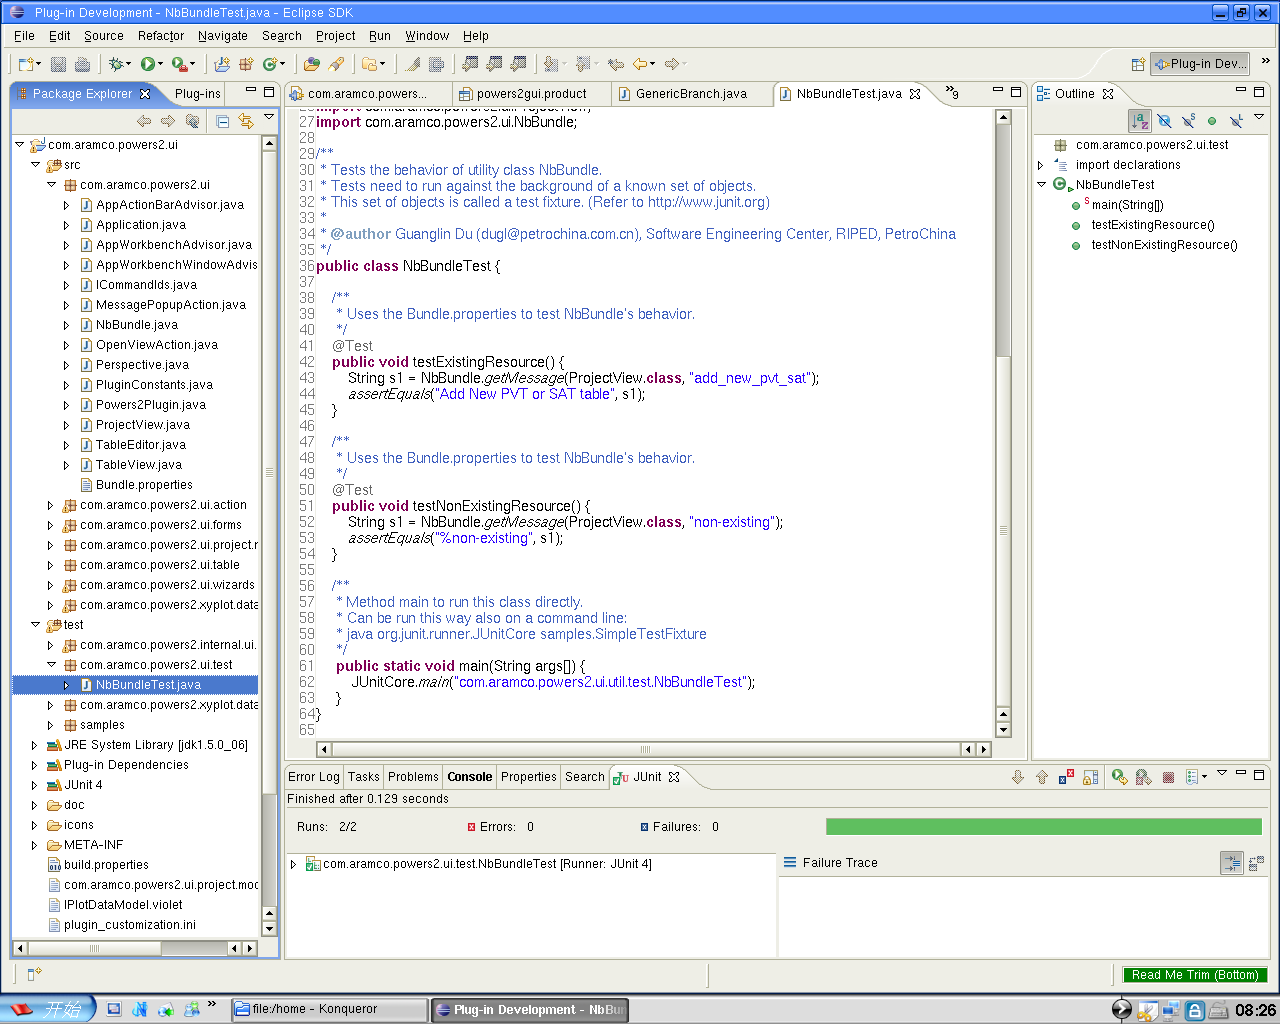
\includegraphics[width=0.5\linewidth]{rys/eclipse1}
  \caption{Środowisko programistyczne Eclipse.}
  \label{fig:schemat}
\end{figure}

\section{{Języki programowania i biblioteki}}

Do zrealizowania aplikacji użyty zostanie język Java. Jest to jeden z najbardziej popularnych języków. 
\cite{horstmann}Java jest językiem, który z założenia miał być prosty, oznacza to, że struktura języka nie jest skomplikowana. Dopatrując się podobieństw, można zauważyć, iż składnia języka jest zbliżona ze składnią C++.  Język ten jest w pełni obiektowy, co w dużej mierze ułatwia projektowanie bardziej złożonych systemów. Twórcy języka postawili również na niezawodność, jednym z argumentów za tym przemawiających jest fakt, iż model wskaźnikowy w tym języku jest zaprojektowany w przemyślany sposób. Nie ma tutaj możliwości nadpisania pamięci i zniszczenia danych, które się w niej znajdują. Mechanizmy abstrakcji zastosowane w tym języku pozwalają na znacznie lepszą i efektywniejszą organizację samego kodu źródłowego, jak również podział logiczny. 


\cite{horstmann}Java ten ma znaczną przewagę na innymi językami programowania,  ze względu na zastosowanie obiektowości oraz ze względu na wiele nowych przydatnych funkcji dodanych w kolejnych odsłonach języka. Z każdą wersją dodawane są nowe funkcjonalności, które w znacznym stopniu ułatwiają pracę programisty. Przestarzałe funkcjonalności są oznaczane jako przestarzałe. Na ich miejsce pojawiają się nowe, co świadczy o tym, iż język ten jest ciągle rozwijany. 


Java dysponuje też pokaźną liczbą gotowych, przygotowanych dla programistów bibliotek. Biblioteki te w większości przypadków wręcz wyręczają programistów. Gotowe rozwiązania znacznie usprawniają i przyspieszają pracę. Umożliwia to zaoszczędzenie dużej ilości czasu poprzez udostępnianie chociażby gotowych rozwiązań z zakresu struktur danych.


Główną zaletą popularności języka jest to, iż istnieje dostęp do dużej liczby kodów źródłowych zawierających gotowe rozwiązania lub opis wraz z rozwiązaniami wielu ważnych problemów pojawiających się stale, przy projektowaniu różnorodnych aplikacji.


\cite{horstmann2}Ważnym aspektem w języka Java jest fakt że programy napisane w tym języku  po kompilacji do plików w formacie obiektowym są uruchamiane na maszynie wirtualnej. Możemy zatem uruchamiać aplikacje na wszystkich urządzeniach które obsługują i mają zainstalowaną Jave. Dzieje się tak dlatego, iż kompilator tworzy kod bajtowy niezależny od żadnego procesora. Kod tak wygenerowany jest tworzony w ten sposób aby jak najszybciej można było go przetłumaczyć na kod maszynowy procesora.


Istotną kwestią przy utrzymywaniu dobrego stylu programowania jest utrzymywanie przejrzystej dokumentacji. Zarządzanie dokumentacją odbywa się przy pomocy narzędzia JavaDoc. Za pomocą znaczników, które umieszczane są w kodzie źródłowym Java jest w stanie wygenerować przejrzystą dokumentację w języku HTML. Używanie znaczników nieznacznie różni się od umieszczania komentarzy. Zostało to rozróżnione, ponieważ nie wszystkie komentarze powinny znajdować się w ogólnej dokumentacji. Blok zdefiniowany na potrzeby Javadoc jest ignorowany przez kompilator. Umieszczenie bloku przed deklaracją klasy lub metody stanowi jej opis. Do dyspozycji zostały oddane również znaczniki umożliwiające opis parametrów poszczególnych metod. 


Zdecydowanie się na konkretny język programowania niesie za sobą decyzje o konkretnych bibliotekach, z którymi praca jest znacznie szybsza, ponieważ zawierają one gotowe rozwiązania. Użyte w projekcje biblioteki to:


\begin{itemize}
\item[•]{jfreechart-1.0.19 jest to bardzo użyteczne narzędzie do tworzenia różnego rodzaju wykresów. W aplikacji główne zastosowanie biblioteka ta znalazła przy generowanie wykresu z pliku dźwiękowego w formacie Wav oraz przy generowaniu wykresu dźwięku w czasie rzeczywistym.}
\item[•]{jMusic1.6.5 jest to biblioteka która, znalazła zastosowanie w drugiej części aplikacji, w której w dużej mierze bazuje się na wykorzystaniu protokołu MIDI. Jej konstrukcja oraz przemyślana funkcjonalność pozwalają na tworzenie logicznych układów nut w protokole MIDI. Dużym ułatwieniem jest także wbudowany konwerter zamieniający podaną wartość w Hercach na odpowiadającą jej nutę.}
\item[•]{TarsosDSP jest to biblioteka zawierająca szeroką gamę zastosowań dotyczących przetwarzania dźwięku.}
\end{itemize}
Realizacja projektu w języku Java pomija problemy związane z obsługą interfejsów dźwiękowych różniących się od siebie w zależności od systemu operacyjnego. Jest to duże ułatwienie, ponieważ każdy system korzysta ze swoich interfejsów takich jak ALSA, JACK oraz OSS w przypadku Linuksa. Wsparcie dla DirectSound and ASIO w przypadku Windowsa oraz SGI w przypadku Macintosha.